\chapter{Previous Studies of Electroweak Physics}
\label{chap:previous}

%TGC Lagrangian: http://www.hep.ucl.ac.uk/~jpc/all/ulthesis/node41.html
%LEP WWZ sensitivity: http://www.hep.ucl.ac.uk/~jpc/all/ulthesis/node43.html

The Glashow-Weinberg-Salam (GWS) theory of electroweak interactions was published in 1968, predicting the existence of $W$ and $Z$ bosons and prompting plans to search for them experimentally.  Indirect evidence for the existence of the $Z$ came in 1973 when the first weak neutral current interactions were observed in the Gargamelle bubble chamber at CERN~\cite{Hasert1973121}.  Direct evidence had to wait until the construction of CERN's Super Proton Synchrotron (SPS) and the observations of the UA1 collaboration in 1983 of first the $W$~\cite{Arnison1983103} and a few months later the $Z$~\cite{Arnison1983398}.  Both observations were quickly confirmed by the competing UA2 collaboration~\cite{Banner1983476,ISI:A1983QT60900027}. The measured masses showed no deviation from the theoretical expectations.

By the end of the 80's, the SPS had been converted into an injector for a new accelerator, the \SI{27}{km} circumference Large Electron-Positron Collider (LEP).  In sharp contrast to the complex $p\bar{p}$ collisions of the SPS where each of the constituent quarks carried energy and could participate in interactions, the $e^+e^-$ collisions at LEP allowed for a new era of clean, high-precision electroweak measurements.  In its first phase, LEP acted as a ``$Z$ factory'', recording 15.5 million $Z$ decays to quarks plus another 1.7 million decays to charged leptons~\cite{Drees:2001xw}.  This high-statistics sample of $Z$ bosons allowed much more precise measurements of the $Z$ mass, width, cross section, and couplings, placing significant new constraints on the electroweak sector of the SM~\cite{:2005ema}.  In its second phase, upgrades allowed the LEP collision energy to surpass the requisite thresholds of \sienergy{160} for $W^+W^-$ production (with observations by all four LEP experiments~\cite{Barate2000205,Abreu200089,Acciarri200019,Abbiendi2000249}) and \sienergy{182} for $ZZ$ production (observed by L3~\cite{Acciarri1999281}).  The LEP experiments were also able to observe $Z\gamma$ events where the photon is radiated from one of the incoming electrons~\cite{Barate:1999tg,Acciarri:2000yu}.  Being an $e^+e^-$ collider, charged final states were forbidden at LEP, excluding any possibility for $WZ$ and $W\gamma$ production.  Nonetheless, the LEP experiments were able to probe the various TGCs through processes involving an off-shell intermediate boson, $e^+ + e^- \to \gamma \to W^+ + W^-$ and $e^+ + e^- \to Z \to W^+ + W^-$ as well as through the process $e^+ + e^- \to e^\pm + W^\mp + \nu$ where a single $W$ is produced through fusion of $W$ and $Z$ bosons radiated from the initial state particles.

The right mixture of design, collision energy, and luminosity to observe $WZ$ events became available only in the final years years of running of Fermilab's Tevatron, a proton-antiproton collider operating at $\sqrt{s}=\SI{1.96}{\TeV}$.  Thus, previous studies of associated $WZ$ events are limited to those conducted by the Tevatron's CDF and \dzero{} experiments, as discussed in the following sections.  CDF and \dzero{} were also able to take measurements of the $W\gamma$ states which had not been previously accessible~\cite{PhysRevLett.94.041803,PhysRevD.71.091108}.

\section{Results from \cdf}
The \cdf collaboration made the first definitive observation of $WZ$ production in 2007, using \SI{1.1}{\fbinv} of collision data~\cite{CDF:WZObservation}.  The collaboration's most recent result measuring the $WZ$ cross section~\cite{Aaltonen:2012vu}, described here, uses \SI{7.1}{\fbinv}.
The analysis identifies $WZ$ candidates by considering events passing a muon or electron trigger with exactly three lepton candidates passing identification requirements and with $\pt > \simomentum{10}$, one of which must satisfy the trigger and a higher \pt requirement (\simomentum{20}) in order to ensure a stable trigger efficiency.  The acceptance for leptons is limited by the instrumented regions to be within a pseudorapidity of 2.0 for electrons and 1.0 for muons.  In order to reduce background contributions, events are also required to have $\MET > \sienergy{25}$. %with the \MET separated by at least $9^\circ$ in azimuth from any substantial jet in the event.  
A $Z$ candidate is chosen based on the pair of same-flavor, opposite-sign leptons for which the invariant mass is closest to the $Z$ mass.  If the best invariant mass differs from the nominal $Z$ mass by more than \simass{15} or if any additional tracks are reconstructed with $\pt > \simomentum{8}$), the event is rejected.  For passing events, the remaining lepton is considered to be from a $W$ decay.

%The \cdf detector includes an inner tracker consisting of silicon microstrips along with an open-cell drift chamber, electromagnetic and hadronic sampling calorimeters, and a muon system consisting of both scintillators and drift chambers.  Due to various gaps in the calorimeter coverage and limited tracking efficiency in the forward region, the acceptance for an analysis which requires three well-identified leptons would be prohibitively low.  To ensure sufficient acceptance, the \cdf analysis distinguishes three separate categories of electrons, three of muons, and an additional category for tracks outside calorimeter acceptance which are also not matched to a muon track.

In performing the cross section measurement, the data must be compared to Monte Carlo (MC) expectations.  For each lepton in MC events, a correction factor is applied to account for measured reconstructions and identification efficiencies.  The largest systematic uncertainties arise from the luminosity measurement (6\%) and the simulated acceptances of the signal ($\approx$ 2.5\%) and background ($\approx$  10\%) processes.  The analysis finds 64 events in the signal region compared to a total expectation of $55.4 \pm 4.9$ events ($8.0 \pm 1.0$ background and $47.4 \pm 4.8$ expected $WZ$ signal).

The final separation between signal and background is achieved through use of a neural network which takes as input various kinematic quantities known to have distributions which differ significantly between the signal and background processes.  The neural network uses MC input to build a single output distribution which maximizes separation between the two regions, with the final cross section $\sigma(p\bar{p} \to WZ) = 3.93^{+0.60}_{-0.53}(\text{stat.})^{+0.59}_{-0.46}(\text{syst.})\,\si{pb}$ extracted with a binned maximum likelihood fit method.

The expected backgrounds for a $WZ$ analysis at CMS come from the same processes considered in this CDF analysis, although the relative importance of the processes differs.  The $ZZ$ process where one of the resulting leptons falls outside detector acceptance represents the primary contribution at CDF, a concern which is less important for CMS where the pseudorapidity coverage is considerably extended and the probability of a missed electron or muon is therefore reduced.  In contrast, the background from \Zjets which is small for CDF becomes a significant concern at CMS due to the high jet multiplicity from pileup collisions (additional low-energy collisions which overlap a collision of interest) at the LHC.  The statistical and systematic uncertainties for this late-stage result from CDF are of comparable magnitude to those achieved in the first results from CMS.

The final state consisting of three leptons along with \MET{} represents only one small slice of the possible decay modes for $WZ$ events.  Although these decays provide the cleanest signatures, it is also possible to look for semi-leptonic signatures with larger branching fractions in events with multiple jets.  Such an analysis suffers from a much larger population of background events which cannot be sufficiently filtered out through simple requirement-based procedures, necessitating the use of more advanced multivariate techniques.  

The decay $W^\pm + Z \to \ell + \nu_\ell + \text{2 jets}$ is virtually indistinguishable from the same process with the $Z$ replaced by a $W$ since the overall charge of the jets cannot be determined.  By considering these two processes together, the CDF collaboration was able to make a measurement of the combined cross section $\sigma(WW) + \sigma(WZ) = 16.0 \pm 3.3\, \si{pb}$ in 2010~\cite{Aaltonen:2009vh}.  The following year, the collaboration published a new study in this channel with a particular emphasis on the invariant mass distribution of the two jets, observing a significant excess of events in the range between \simass{120} and \simass{160}~\cite{Aaltonen:2011mk} which can be interpreted in various new physics models including Technicolor~\cite{Eichten:2012br}.  The results from CMS presented in Chapter~\ref{chapter:limits}, however, rule out this Technicolor interpretation.

%This analysis found 16 events in the signal region compared to a background expectation of $2.7 \pm 0.4$ events.  The cross-section measurement is performed with a maximum likelihood fit in two \MET bins with a measured result that $\sigma(WZ) = 5.0^{+1.8}_{-1.4} \text{(stat.)} \pm 0.4 \text{(syst.)} \pb$.  The NLO prediction for the $WZ$ cross-section in $p\bar{p}$ collisions at $\sqrt{s}=1.96\TeV$ relevant to this analysis is $3.7 \pm 0.3 \pb$~\cite{Campbell:1999ah} where the uncertainty includes a 3\% effect from the choice of parton distribution function and a 7\% effect from the choice of scale used in the calculations (assumed as the average vector boson mass).  CDF's experimental result confirms the theoretical prediction but the large statistical uncertainty means that the result is not able to place any significant new contraints on the Standard Model.

\section{Results from \dzero}
%The \dzero detector contains a central silicon microstrip/fiber tracking system surrounded by a \SI{2}{T} superconducting solenoidal magnet, electromagnetic and hadronic uranium-liquid argon sampling calorimeters, and a muon system of drift tubes and scintillation counters surrounded by a \SI{1.8}{T} toroidal magnet.

The other major Tevatron experiment, \dzero, took measurements of \wztolnll with \SI{4.1}{\fbinv} of data~\cite{D0:2010qn} and placed the first limits on \wprime models with decays to $WZ$ \cite{D0:2009eu}.
For the cross section measurement, $WZ$ candidate events are required to contain at least three lepton candidates passing identification criteria and with $\pt > \simomentum{15}$ which are also separated by at least 0.5 in $\Delta R$, defined as:
\begin{equation}
  \label{eq:deltar}
  \Delta R = \sqrt{(\Delta\phi)^2 + (\Delta\eta)^2}.
\end{equation}
A $Z$ candidate is chosen based on the pair of same-flavor, opposite-sign leptons for which the invariant mass is closest to the $Z$ mass.  Of the remaining leptons, the one with the highest transverse momentum is assigned to the $W$, with a minimum \MET of \sienergy{20} required to further support the $W$ hypothesis.  For the resonance search, the same basic selection is modified to focus on higher-energy events, raising the lepton \pt requirement to \simomentum{20} and the \MET requirement to \sienergy{30} while demanding that the lepton assigned to the $W$ be separated by at least 1.2 in $\Delta R$ from each of the $Z$ leptons.

Employing a likelihood method to combine results from each of the four leptonic $WZ$ decay channels, \dzero measures $\sigma(WZ) = 3.90^{+1.01}_{-0.85} \text{(stat. + syst.)} \pm 0.31 \text{(lumi.)}\,\pb$ with uncertainties dominated by the available collision statistics.  The analysis finds 34 candidate events, compared to an expected $23.3 \pm 1.5$ signal and $6.0 \pm 0.6$ background events.  These results are in agreement with an NLO prediction of $3.25 \pm \SI{0.19}{pb}$~\cite{Campbell:1999ah} by the same method as discussed for CDF.

\begin{figure}
  \centering
  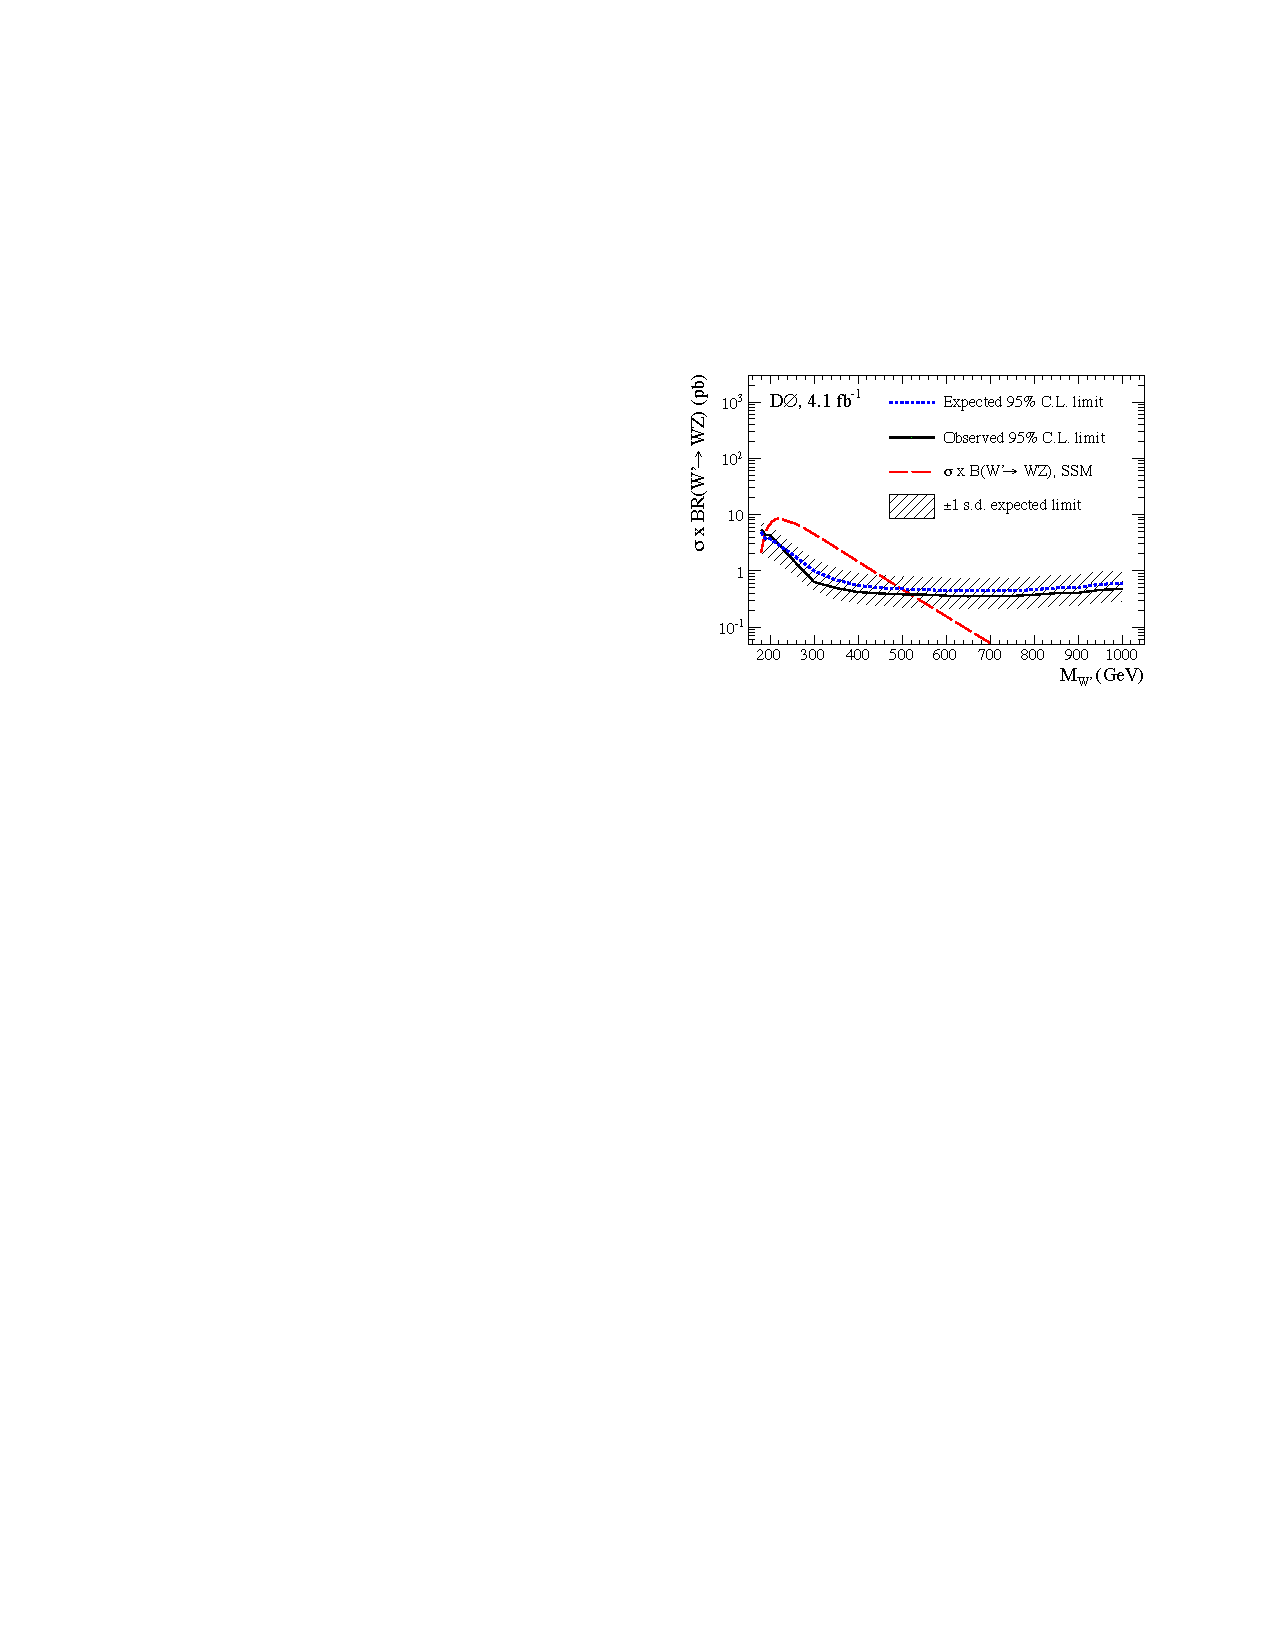
\includegraphics{figures/d0limit-wprime}
  \caption[\wprime limits from \dzero]{Limits on the cross section for \wprime production in the SSM based on results from \dzero{}.}
  \label{fig:d0limit-wprime}
\end{figure}

\begin{figure}
  \centering
  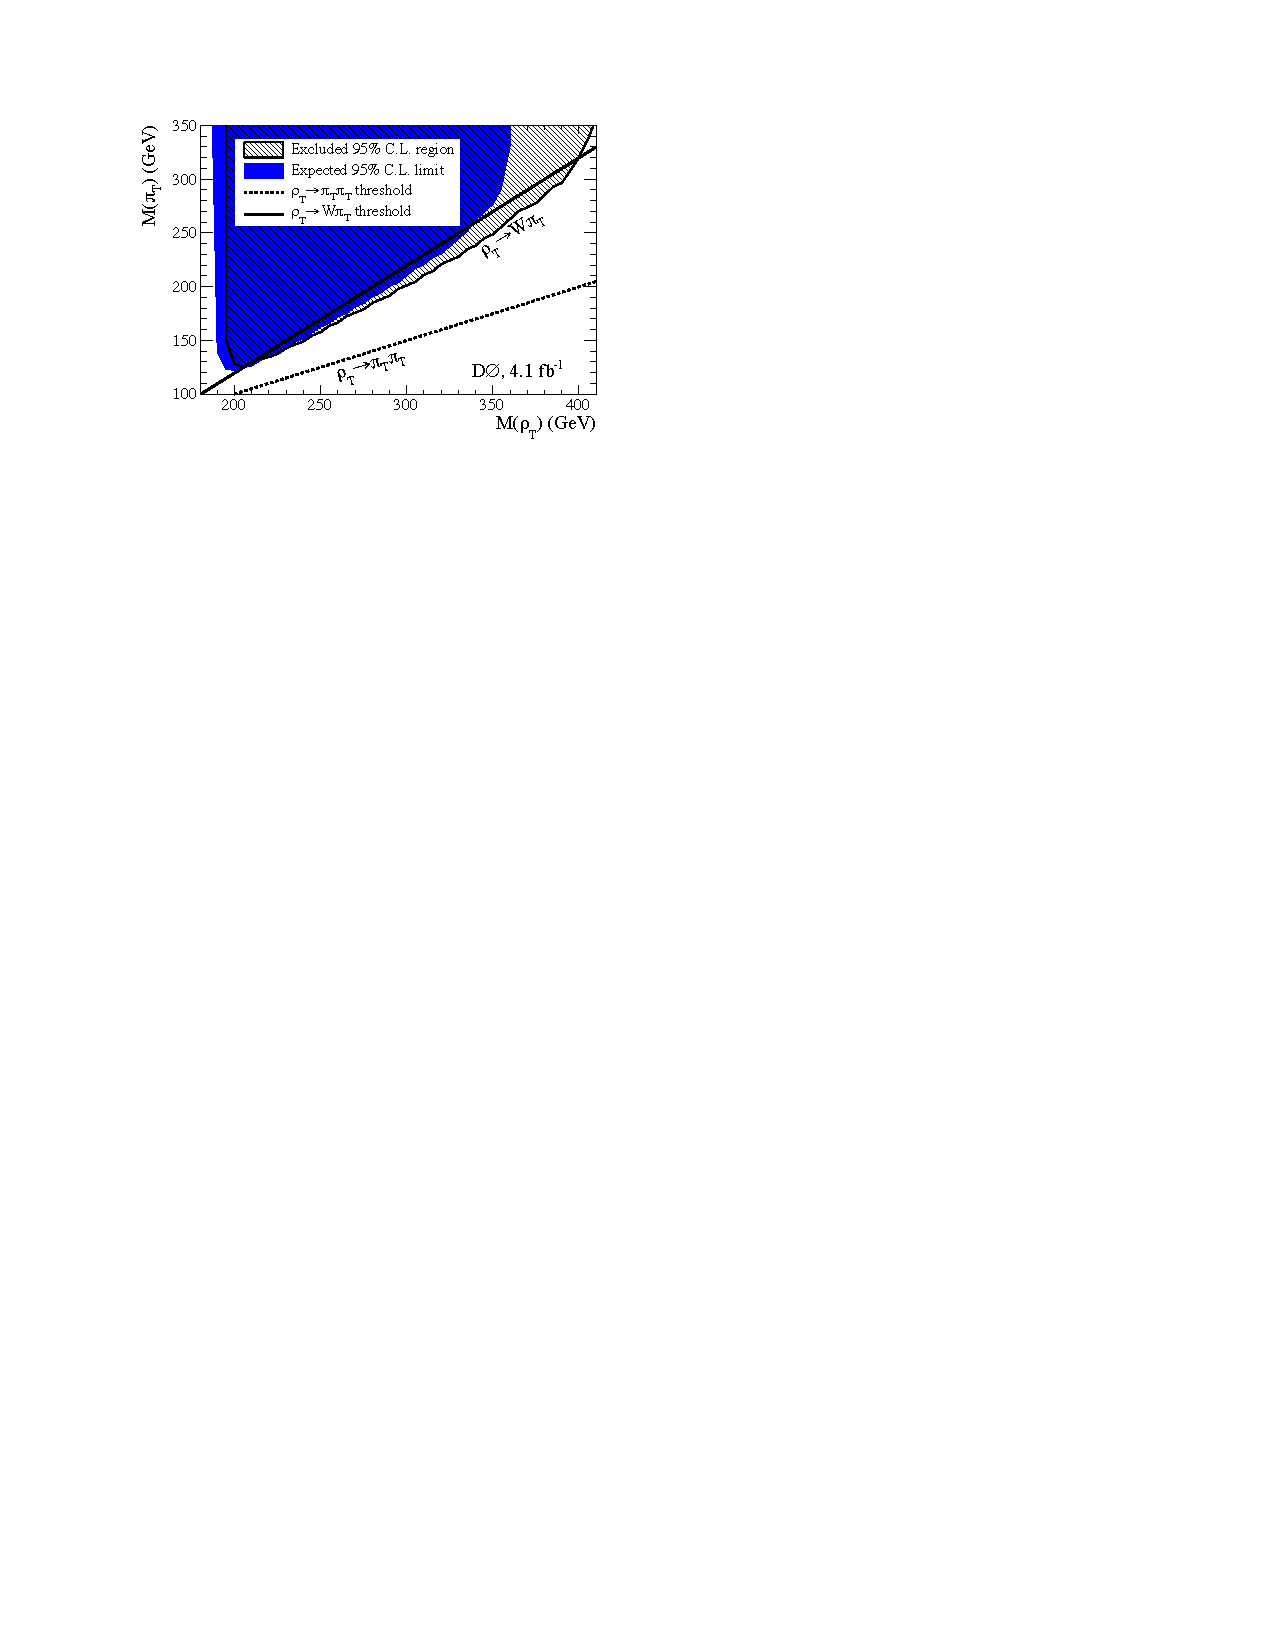
\includegraphics{figures/d0limit-tc}
  \caption[Technicolor limits from \dzero]{Excluded regions of technicolor parameter space based on results from \dzero{} with the thresholds of the $\technirho \to W + \technipi$ and $\technirho \to \technipi + \technipi$ decays overlaid.}
  \label{fig:d0limit-tc}
\end{figure}

For the resonance search, seeing that the number of observed events is consistent with SM predictions, the analysis proceeds to set limits on \wprime and technicolor models using a modified frequentist approach.  The limit-setting procedure relies on the transverse mass of the $WZ$ system to discriminate between signal and background, leading to results shown in Figures~\ref{fig:d0limit-wprime} and~\ref{fig:d0limit-tc}.  Within the SSM, they exclude a \wprime with mass in the range \simass{188} to \simass{520} at 95\% confidence level and find their results hold well in models with increased width of the \wprime{}.  Within technicolor models, they exclude a \technirho with mass in the range \simass{208} to \simass{408} under the assumption $M(\technirho) < M(\technipi) + M(W)$.

A comparison of this \dzero{} study to the potential for measurements at CMS closely follows the comparison made to CDF above.  The primary background at \dzero{} is from $ZZ$ rather than \Zjets and their cross section sensitivity is comparable to what has been achieved in the first results from CMS.  The higher energy of the LHC, however, makes a substantial difference in the reach for resonance searches with CMS, ruling out new sections of \wprime{} and Technicolor parameter space as discussed in Chapter~\ref{chapter:limits}.

% TODO: Talk about ATLAS results.

